\documentclass[pagenumber=off]{article}

\usepackage[pdftex]{graphicx}
\usepackage{xcolor}
\usepackage[a4paper,margin=0.7in,portrait]{geometry}
\usepackage{etoolbox}
\usepackage{hyperref}

%----------------------------------------------------------
\definecolor{coolblack}{rgb}{0.0, 0.18, 0.39}
%\AtBeginDocument{\color{coolblack}}
%----------------------------------------------------------

%%----------------------------------
\begin{document}

%%--- Title ---
\begin{titlepage}
\begin{center}
\vspace{1cm}
{\textcolor{gray}\today}\\
{\textcolor{gray}{\bf Udacity Nanodegree: Deep Reinforcement Learning }}\\
\vspace{1.5cm}
{\textcolor{coolblack}{\huge \bf III Project: Collaboration and Competition}}\\
\vspace{0.5cm}
{\textcolor{coolblack}{\Large \bf  Learning to play tennis via Multi Agent Reinforcement Learning}}
\par
\vspace{0.5cm}
%{\textcolor{coolblack}{\Large\itshape Solved using Deep Deterministic Policy Gradient (DDPG).}}\par
\vspace{6cm}
\end{center}
\tableofcontents

\vspace{4cm}

\begin{center}
{Alberto M. Cozzini}\\
\end{center}
\end{titlepage}

%----------------------------------
\section{Task}
For this project, an agent has to learn to control a double-jointed arm to reach target locations.\\
A reward of +0.1 is provided for each step that the agent's hand is in the target location. The objective is to track the target location for as many time steps as possible.

The task is episodic and in order to solve the environment the agent/s must get an average score of at least +30 over 100 consecutive episodes. Here is an example of benchmark solution.
%----------------------------------
\begin{figure}[!h]
  \centerline{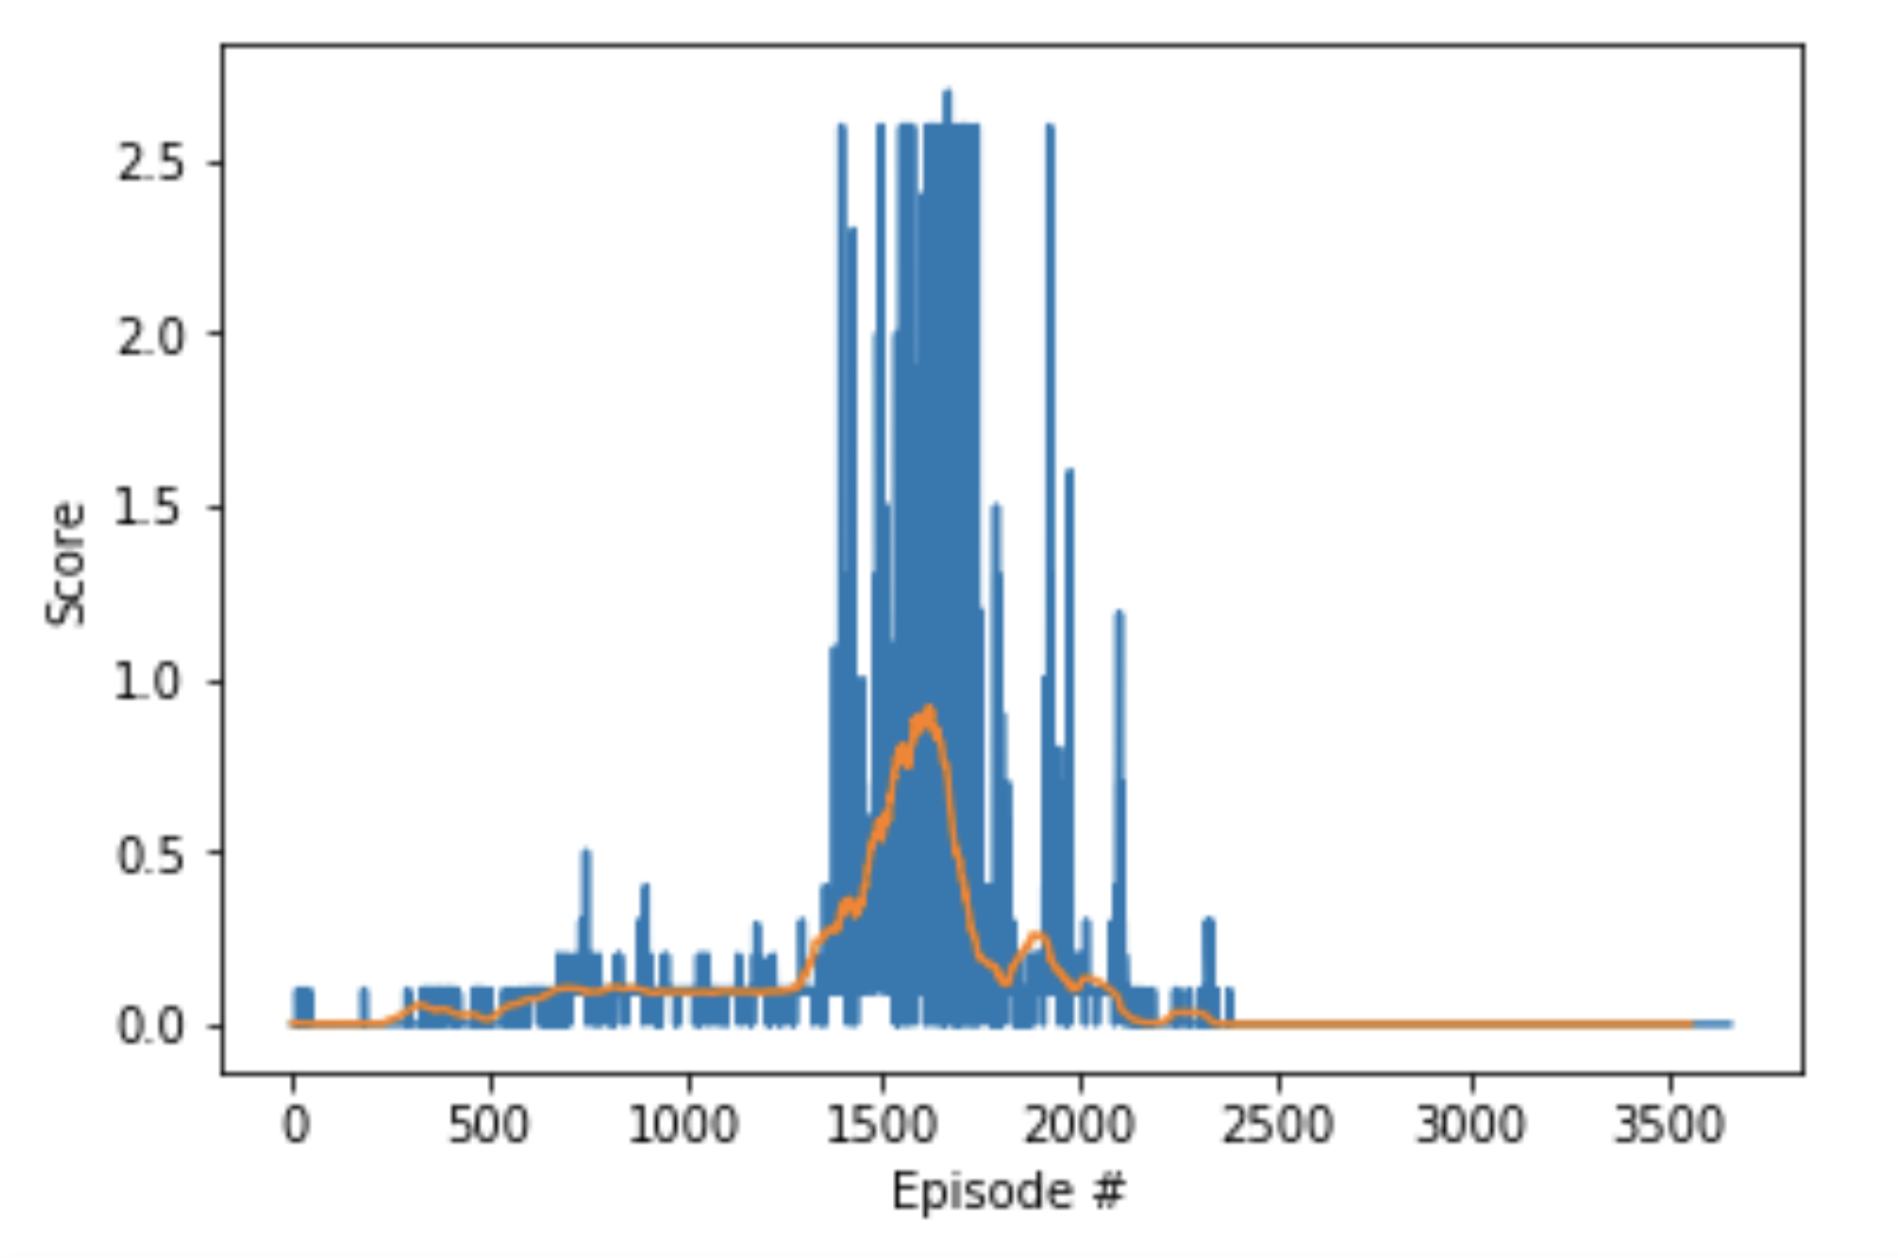
\includegraphics[page=1, height=6cm, width=12 cm, angle=0]{./Plots/Benchmark_Score.png}}
  \caption{Benchmark Implementation. It reaches an average score of at least 30 over about 100 episodes.}
\end{figure}
%----------------------------------

%----------------------------------
\section{Environment}
The environment is built on Unity architecture.\\
The state space consists of 33 variables representing position, rotation, velocity, and angular velocities of the arm. 
Given this information, the agent has to learn how to best select actions. Each action is a four dimensional vector, corresponding to torque applicable to the two joints. Each scalar in the action vector should be a number bounded between -1 and 1.

\subsection{Discount Factor}
The utility function of the agent values the immediate reward more than the futures rewards which are discounted at a factor of 0.99 per time step.


\section{Learning Algorithm} 
The agent objective is to learn by interacting with the environment.\\
To speed up the learning process we use 20 clones of the same agent learning simultaneously from shared experiences.

We implement a Deep Deterministic Policy Gradient (DDPG) as per the paper \href{https://arxiv.org/abs/1509.02971}{Continuous control with deep reinforcement learning}. It is an off-policy actor-critic model free algorithm based on the deterministic policy gradient that can extended the advantaged of the standard deep Q-Learning to continuous action space.


\subsection{Loss Function}

As in Q-Learning, by the Bellman equation, the loss function for the critic network is the mean square error between the expected Q values computed on the local network and the target Q values computed on the network with momentarily frozen weights.  

The actor policy is updated using the sample policy gradient. We use the local policy network to find the optimal action given the state and then we feed it to our local Q-value function, which is what we want to maximise. 

\subsubsection{Optimizer}

The optimizer performs a stochastic gradient descent step on the loss function with respect to the network weights.\\
We implement the Adam optimization algorithm with learning rate of 1e-3.\\


\subsubsection{Critic Gradient Clipping}

As suggested by the course notes, we tested the extra stabilizing option of clipping the gradient when training the critic network.


\subsubsection{Soft Update}

To improve stability of learning process and avoid oscillations, we keep separate local and target networks. While the two networks are identical clones, we only update the weights of the target network by interpolating old with new local weights by a factor of 1e-3.

\subsubsection{Periodic Update}

We tested without success the periodic update  


\subsection{Decaying Action Noise}
We need to add noise to our actions to force exploration. Nonetheless we want to force a decay of the noise with time.
The temporally correlated noise is generated via Ornstein-Uhlenbeck process with drift $\theta=0.1$ and volatility $\sigma=0.2$ decays by a factor $\epsilon=0.99$ after each episode.


\subsection{Experience Replay}
To make the learning process more stable and avoid aberration of the action-value Q function, we store and randomly replay some of the recent buffer of experiences, 1e5.
The number of experiences we store in hour memory is 1e5. Each time we sample uniformly at random a batch of 128. We tested a bigger buffer, 256, which yield a slightly higher performance with marginally slower learning curve.




%-------------------------------
\section{Model Architecture}

We have two separate neural networks to approximate non linear functions representing the actor function and the critic action-value function. 

\subsection{Actor}
The input is the array of the 33 state observations.
The network has two hidden layers. Each hidden layer has fully connected 128 nodes.
We use the leaky ReLU activation function which has the benefit of having a very small slope for $x < 0$.
The output is mapping to the 4 continuous actions with tangent activation function to bound each between -1 and +1.

\subsection{Critic}
The critic network approximates the Q-value function for a given state and action.
It has two fully connected hidden layers each of 128 nodes.
In this instance we use again the Leaky ReLU activation function.

\subsection{Dropout}
To make the network more robust we tested without success to implement a Dropout step, where randomly a small percentage of nodes are drop from a learning iteration.


\newpage
%----------------------------------
\section{Solved}

After less than 60 episodes (60,000 agent steps) the average score across all agents is already above 30.
It reaches a plateau around 37 which is steadily maintained for the following 100 episodes without any major slip.

\begin{table}[h]
  \centering
    \begin{tabular}{|l|c|c|}
      \hline
      {\bf Episode} & {\bf \# Steps} & {\bf Avg. Score} \\ 
      \hline
      10 & 10,000 & 0.78 \\
      20 & 20,000 & 2.49 \\
      30 & 30,000 & 7.93 \\
      40 & 40,000 & 13.85 \\
      50 & 50,000 & 22.93 \\
      {\bf  60} & {\bf 60,000} & {\bf 34.79} \\
      70 & 70,000 & 37.83 \\
      80 & 80,000 & 36.99 \\
      90 & 90,000 & 37.55 \\
      100 & 100,000 & 37.80 \\
      110 & 110,000 & 36.22 \\
      120 & 120,000 & 37.78 \\
      130 & 130,000 & 38.19 \\
      140 & 140,000 & 37.22 \\
      \hline
      {\bf 150} & {\bf 150,000} & {\bf 37.31} \\      
      \hline
    \end{tabular}
    \caption{Rolling average score over all 20 agents.}
  \end{table}

\vspace{-1cm}
%----------------------------------
\begin{figure}[!h]
  \centerline{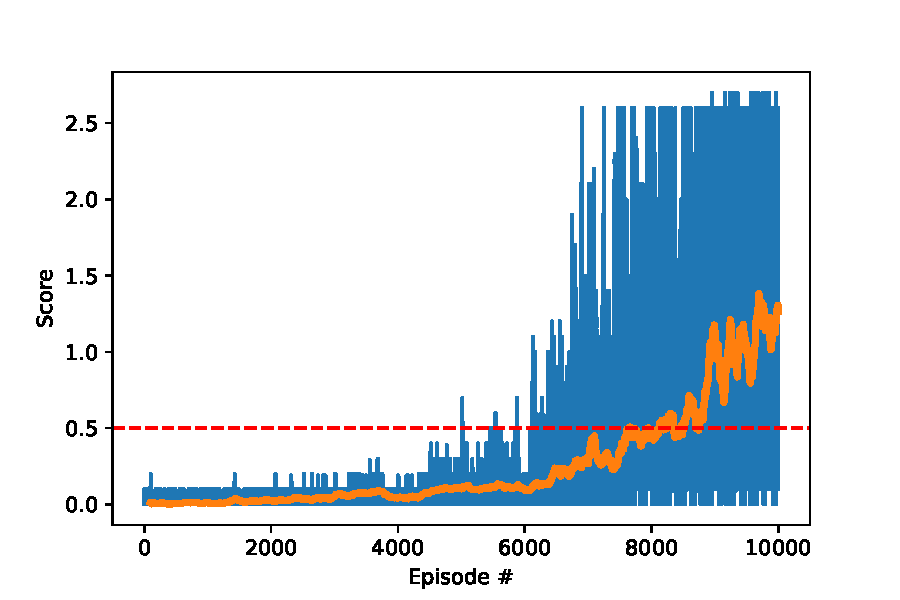
\includegraphics[page=1, height=8cm, width=14cm, angle=0]{./Plots/Average_Score.pdf}}
  \caption{Average score by episode.}
\end{figure}

%----------------------------------


%\newpage
%----------------------------------
\section{Future Work}

The current solution is already quite efficient in reaching its target in reasonably number of episodes.
Nonetheless, looking at possible ways to improve the current architecture there would be few options.

Prioritized experience replay. We are currently uniformly sampling from past experiences, but a likely improvement would be to prioritize samples that yielded greater weights updated, i.e. greater TD error.

One improvement suggested is to add noise directly to the network weights instead of shocking the action vector.

Of the more recent algorithms one that could be interesting to try out is the Guided Policy Search (GPS) which has been proven to be data efficient and quite successful in robots control problems, even if the current task is not vision driven. 

\end{document}
